\section{Jawaban}

%=========================================================%
%                  TULIS JAWABAN DI SINI                  %
% Jangan Lupa untuk Menghapus Contoh Jawaban di Bawah Ini %
%=========================================================%

\subsection{Jawaban Pertanyaan 1}

Misalnya di sini akan dibuatkan variabel tambahan berupa \inlinesnippet{x}, \inlinesnippet{size}, dan \inlinesnippet{peluang} dengan isi angka sesuai dengan yang ada di soal --- tujuannya supaya angka tersebut bisa dipakai lagi untuk ditampilkan di teks terminal. Adapun \textit{command/script} yang digunakan serta \textit{output}-nya akan ditampilkan sebagai berikut:

\clearpage

\begin{lstlisting}[
    caption={Matriks Data Binomial}, 
    language=R, 
    basicstyle=\small\ttfamily
]
cat("\n\n---------- [ Pertanyaan 1 ] ----------\n\n")

n <- 30
size <- 10
peluang <- 0.3
data_binomial <- matrix(rbinom(n, size = size, prob = peluang), ncol = 5)

cat(paste0("Matriks Data Binomial --> 𝑛 = ", n, ", size = ", size, ", 𝑝 = ", peluang, "\n"))
print(data_binomial)
\end{lstlisting}

\begin{figure}[H]
    \centering
    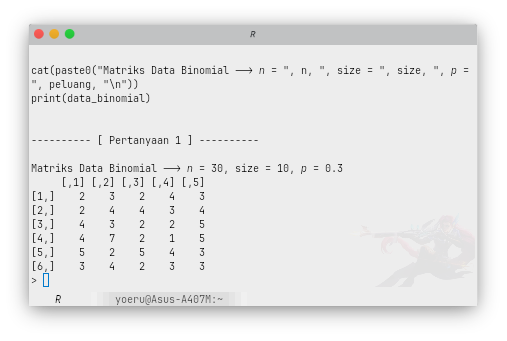
\includegraphics[width=.8\linewidth]{image/Matriks Data Binomial.png}
    \vspace{-\baselineskip}
    \caption{Tampilan Terminal Kode 1---Matriks Data Binomial}
\end{figure}

\begin{lstlisting}[
    caption={\textit{Output} dari Kode 1---Matriks Data Binomial}, 
    basicstyle=\small\ttfamily
]
---------- [ Pertanyaan 1 ] ----------

Matriks Data Binomial --> 𝑛 = 30, size = 10, 𝑝 = 0.3
     [,1] [,2] [,3] [,4] [,5]
[1,]    2    3    2    4    3
[2,]    2    4    4    3    4
[3,]    4    3    2    2    5
[4,]    4    7    2    1    5
[5,]    5    2    5    4    3
[6,]    3    4    2    3    3
\end{lstlisting}

\subsection{Jawaban Pertanyaan 2}

Di sini akan dibuatkan variabel \inlinesnippet{derajat_bebas} dan \inlinesnippet{x} yang menyimpan isi angka sesuai pada soal, kemudian isi data chisquare akan disimpan sebagai objek/variabel bernama \inlinesnippet{data_chisquare} --- supaya data dan angka tersebut mudah dipanggil saat pembuatan \textit{plot}-nya. Berhubung saya menggunakan \textit{OS} basis Linux, \textit{device} grafiknya memakai \inlinesnippet{x11()}.

Akan tetapi, ada keanehan dengan soal tersebut. Di soal meminta dengan derajat bebas 10, sedangkan hasil grafik yang ditunjukkan di soal tersebut justru menampilkan grafik dengan derajat bebas 1 (bagian judul “df=1”). Oleh karenanya, saya akan buatkan dua jenis jawaban, yaitu dengan asumsi  \inlinesnippet{derajat_bebas <- 10}  dan dengan asumsi  \inlinesnippet{derajat_bebas <- 1}.

\subsubsection{Asumsi 1 --- Derajat Bebas 10 (\texttt{df = 10})}

Hasil grafik yang akan ditampilkan akan jauh berbeda dari contoh hasil grafik yang diberikan pada soal. Adapun \textit{command/script} yang digunakan beserta \textit{output} terminal dan \textit{output} grafik akan ditampilkan sebagai berikut.

\begin{lstlisting}[
    caption={Data Kepadatan Chisquare dengan Derajat Bebas = 10}, 
    language=R, 
    basicstyle=\small\ttfamily
    ]
# Pertanyaan 2 #
cat("\n\n---------- [ Pertanyaan 2 ] ----------\n\n")

# Asumsi df = 10 (sesuai soal, tapi tidak sesuai dengan contoh grafiknya)
derajat_bebas <- 10
x <- seq(0, 5, length.out = 100)
data_chisquare <- dchisq(x, derajat_bebas)

x11()
plot(x, data_chisquare,
type = "l",
xlab = "x",
ylab = "Kerapatan",
main = paste0("Distribusi Chisq:  𝑑𝑓 = ", derajat_bebas))

cat(paste0("Grafik Kepadatan Chisquare Sudah Ditampilkan --> df = ", derajat_bebas, "\n"))

# Asumsi df = 1 (sesuai dengan contoh grafiknya, tapi tidak sesuai soal)
derajat_bebas <- 1
data_chisquare <- dchisq(x, derajat_bebas)

x11()
plot(x, data_chisquare,
type = "l",
xlab = "x",
ylab = "Kerapatan",
main = paste0("Distribusi Chisq:  𝑑𝑓 = ", derajat_bebas))

cat(paste0("Grafik Kepadatan Chisquare Sudah Ditampilkan --> df = ", derajat_bebas, "\n"))
\end{lstlisting}

\begin{figure}[H]
    \centering
    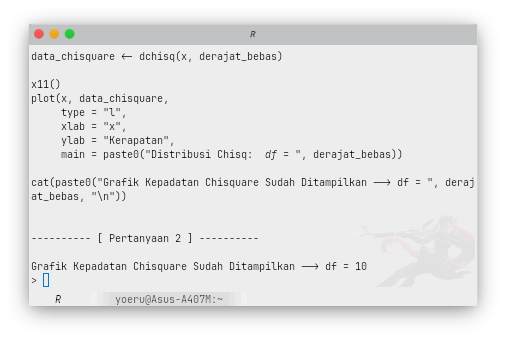
\includegraphics[width=.8\linewidth]{image/Kepadatan Chisquare df10.png}
    \vspace{-\baselineskip}
    \longcaption{Terminal Kode 3---Kepadatan Chisquare \\ dengan Derajat Bebas 10}
\end{figure}

\begin{figure}[H]
    \centering
    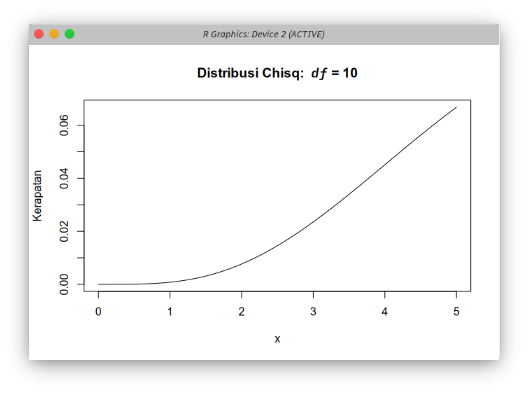
\includegraphics[width=.8\linewidth]{image/Grafik Kepadatan Chisquare Berderajat Bebas 10.png}
    \vspace{-\baselineskip}
    \longcaption{\textit{Output} Kode 3---Grafik Kepadatan Chisquare \\ dengan Derajat Bebas 10}
\end{figure}

\subsubsection{Asumsi 2 --- Derajat Bebas 1 (\texttt{df = 1})}

Hasil grafik yang akan ditampilkan bisa mirip dengan contoh grafik yang diberikan pada soal. Bagian ini masih memanfaatkan objek yang dibuat sebelumnya, hanya saja bagian \inlinesnippet{derajat_bebas} diubah menjadi 1 dan sisanya dipanggil kembali seperti biasanya. Adapun \textit{command/script} yang digunakan beserta \textit{output} terminal dan \textit{output} grafik akan ditampilkan sebagai berikut.

\begin{lstlisting}[
    caption={Data Kepadatan Chisquare dengan Derajat Bebas = 1}, 
    language=R, 
    basicstyle=\small\ttfamily
]
# Asumsi df = 1 (sesuai dengan contoh grafiknya, tapi tidak sesuai soal)
derajat_bebas <- 1
data_chisquare <- dchisq(x, derajat_bebas)

x11()
plot(x, data_chisquare,
type = "l",
xlab = "x",
ylab = "Kerapatan",
main = paste0("Distribusi Chisq:  𝑑𝑓 = ", derajat_bebas))

cat(paste0("Grafik Kepadatan Chisquare Sudah Ditampilkan --> df = ", derajat_bebas, "\n"))
\end{lstlisting}

\begin{figure}[H]
    \centering
    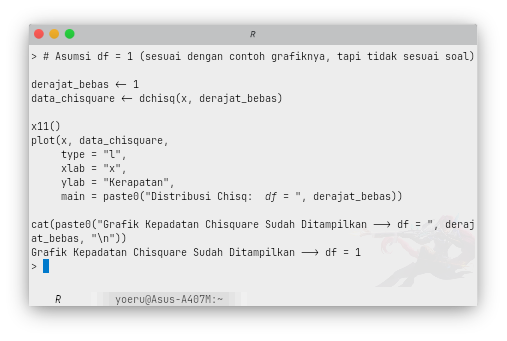
\includegraphics[width=.8\linewidth]{image/Kepadatan Chisquare df1.png}
    \vspace{-\baselineskip}
    \longcaption{Terminal Kode 4---Kepadatan Chisquare \\ dengan Derajat Bebas 1}
\end{figure}

\begin{figure}[H]
    \centering
    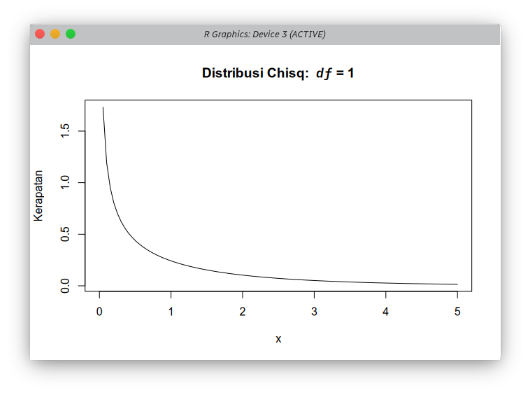
\includegraphics[width=.8\linewidth]{image/Grafik Kepadatan Chisquare Berderajat Bebas 1.png}
    \vspace{-\baselineskip}
    \longcaption{\textit{Output} Kode 4---Grafik Kepadatan Chisquare \\ dengan Derajat Bebas 1}
\end{figure}

\subsection{Jawaban Pertanyaan 3}

\subsubsection{Program 1 --- Perkiraan Peluang Kemenangan \textit{Game Online} dengan Distribusi Logistik}

Pada contoh program ini akan dibuat tabel dan grafik tentang perkiraan peluang untuk bisa menang di \textit{game online} dengan memakai fungsi distribusi logistik berupa \inlinesnippet{plogis()}. Contoh program ini terinspirasi dari kejadian dan istilah tertentu yang bisa ditulis seperti: \textit{“kalau jarang main, biasanya sistem selalu kasih menang ke pemain itu. Akan tetapi, kalau keseringan main hingga terlalu candu, sistem akan membuatnya sering kalah untuk memaksanya beristirahat”}

Variabel yang dibuat yaitu \inlinesnippet{frekuensi_game} yang berisi 100 angka dari rentang 1 sampai 40 (asumsi main hingga mencapai 40 \textit{match} dalam seharian adalah batas yang mulai tidak wajar), \inlinesnippet{peluang_tengah} yang menentukan posisi \textit{match} dengan peluang menang di 50\% (di sini, \textit{match} ke-15 sebagai peluang tengah), dan \inlinesnippet{scale} yang menentukan \textit{keluwesan} dari perubahan peluangnya (semakin \textit{luwes}, penurunan peluang juga semakin halus).

\begin{lstlisting}[
    caption={Distribusi Logistik untuk Peluang Kemenangan dalam \textit{Game Online}}, 
    language=R, 
    basicstyle=\small\ttfamily
]
# Pertanyaan 3 #
cat("\n\n---------- [ Pertanyaan 3 ] ----------\n\n")

cat("Program 1 | Peluang Kemenangan dalam Game Online [Distribusi Logistik]\n\n")

frekuensi_game <- seq(1, 40, length.out = 100)
peluang_tengah <- 15
scale <- 4
data_peluang_logistik <- 1 - plogis(frekuensi_game, peluang_tengah, scale)

# Tabel
tabel_peluang_logistik <- data.frame("Match" = 1:40, "Peluang.Menang" = paste0(abs(round(1 - plogis(40:1, peluang_tengah, scale) * 100, 2)), "%"))
print(tabel_peluang_logistik, row.names = FALSE)

# Grafik
x11()
plot(frekuensi_game, data_peluang_logistik,
type = "l",
xlab = "Game/Match per Hari",
ylab = "Peluang untuk 'Dikasih Menang'",
yaxt = "n",
col = "red",
main = paste0("Peluang Kemenangan Game Online | Dist. Logistik: μ = ", peluang_tengah, ", 𝒔 = ", scale),
sub = "(Semakin Sering Main, Semakin Rendah Peluang Kemenangannya)")

axis(side = 2, at = seq(0, 1, by = 0.2), labels = paste0(seq(0, 1, by = 0.2) * 100, "%"), las = 1)
\end{lstlisting}

\begin{figure}[H]
    \centering
    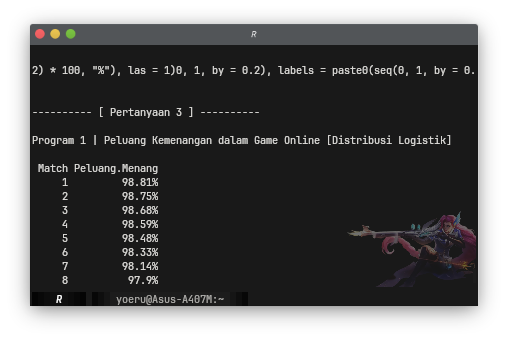
\includegraphics[width=.8\linewidth]{image/Peluang Kemenangan dalam Game Online dengan Distribusi Logistik.png}
    \vspace{-\baselineskip}
    \longcaption{Terminal Kode 5---Peluang Kemenangan dalam \\ Game Online dengan Distribusi Logistik}
\end{figure}

\begin{figure}[H]
    \centering
    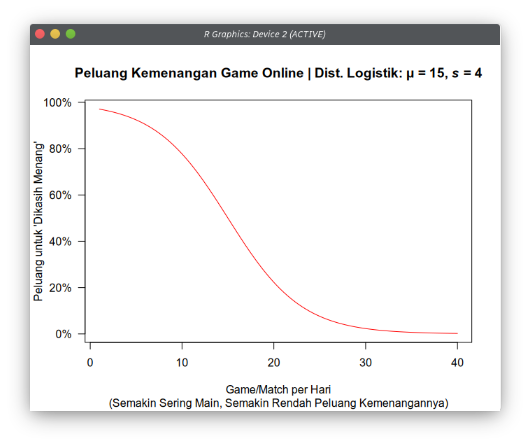
\includegraphics[width=.8\linewidth]{image/Grafik Peluang Kemenangan dalam Game Online dengan Distribusi Logistik.png}
    \vspace{-\baselineskip}
    \longcaption{\textit{Output} Kode 5---Grafik Peluang Kemenangan dalam \\ Game Online dengan Distribusi Logistik}
\end{figure}

\subsubsection{Program 2 --- Perkiraan Kecemasan Seseorang di Sekitar Waktu Ujian dengan Distribusi Normal}

Pada contoh program ini akan dibuat grafik tentang perkiraan tingkat kecemasan seseorang dalam waktu-waktu tertentu untuk menghadapi ujian dengan memakai fungsi distribusi normal berupa \inlinesnippet{dnorm()}. Variabel yang akan dibuat yaitu \inlinesnippet{waktu} yang berisi rentang dari -6 sampai 6 (-6 sebagai 6 jam sebelum ujian, +6 sebagai 6 jam setelah ujian), \inlinesnippet{puncak_kecemasan} yang menentukan puncak kecemasan di posisi jam tertentu (di sini puncaknya adalah saat +1 karena biasanya seseorang mulai cemas di jam tersebut karena khawatir jawabannya tidak selesai setelah waktu habis), dan \inlinesnippet{sebaran_kecemasan} yang menentukan seberapa halus/seberapa dadakan perubahan kecemasan tersebut (di sini pilihnya 1,6).

\begin{lstlisting}[
    caption={Perkiraan Kecemasan Seseorang di Sekitar Waktu Ujian dengan Distribusi Normal}, 
    language=R, 
    basicstyle=\small\ttfamily
]
cat("\n\nProgram 2 | Tingkat Kecemasan di Sekitar Waktu Ujian [Distribusi Normal]\n\n")

waktu <- seq(-6, 6, by = 0.1)
puncak_kecemasan <- 1
sebaran_kecemasan <- 1.6
data_kecemasan_normal <- dnorm(waktu, puncak_kecemasan, sebaran_kecemasan)

x11()
plot(waktu, data_kecemasan_normal,
type = "l",
col = "darkred",
lwd = 2,
xlab = "Waktu Relatif",
ylab = "",
ylim = c(0, 0.3),
main = paste0("Kecemasan Seseorang di Sktr. Wktu. Ujian | Dist. Normal: μ = ", puncak_kecemasan, ", σ = ", sebaran_kecemasan),
sub = "(Sebelum ⟵ | ⟶ Sesudah)",
xaxt = "n",
yaxt = "n")

axis(side = 2, at = seq(0, 0.3, by = 0.05), labels = paste0("+", seq(0, 0.3, by = 0.05) * 100, "%"), las = 1)
axis(side = 1, at = c(-6, -4, -2, 0, 2, 4, 6), labels = c("-6 Jam", "-4 Jam", "-2 Jam", "Ujian Mulai", "+2 Jam", "+4 Jam", "+6 Jam"), las = 1)
grid(col = "lightgray", lty = "dotted")

cat(paste0("Grafik Sudah Ditampilkan --> μ = ", puncak_kecemasan, ", σ = ", sebaran_kecemasan, "\n\n"))
\end{lstlisting}

\begin{figure}[H]
    \centering
    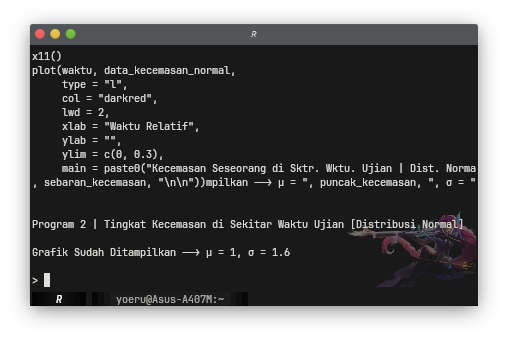
\includegraphics[width=.8\linewidth]{image/Kecemasan Seseorang di Sekitar Waktu Ujian dengan Distribusi Logistik.png}
    \vspace{-\baselineskip}
    \longcaption{Terminal Kode 6---Perkiraan Kecemasan Seseorang \\ di Sekitar Waktu Ujian dengan Distribusi Normal}
\end{figure}

\begin{figure}[H]
    \centering
    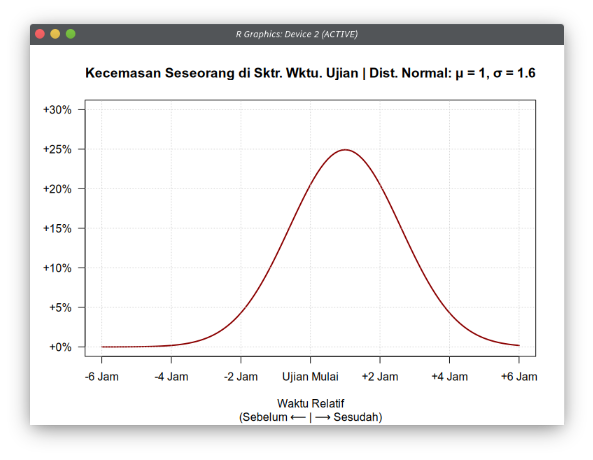
\includegraphics[width=.8\linewidth]{image/Grafik Kecemasan Seseorang di Sekitar Waktu Ujian dengan Distribusi Logistik.png}
    \vspace{-\baselineskip}
    \longcaption{\textit{Output} Kode 6---Grafik Perkiraan Kecemasan Seseorang \\ di Sekitar Waktu Ujian dengan Distribusi Normal}
\end{figure}

\subsection{\textit{Script} dan \textit{Output} Keseluruhan}

Di bagian ini akan ditampilkan script dan output terminal secara keseluruhan --- dari bagian nama \& UPBJJ hingga contoh program yang dibuat. 

\subsubsection{Script}

\begin{lstlisting}[language=R, numbers=left, basicstyle=\small\ttfamily]
# Komputer I
# Diskusi 7


# Nama & UPBJJ #
cat("Nama  : Yoeru Sandaru\n")
cat("UPBJJ : UT Jakarta\n")


# Pertanyaan 1 #
cat("\n\n---------- [ Pertanyaan 1 ] ----------\n\n")

n <- 30
size <- 10
peluang <- 0.3
data_binomial <- matrix(rbinom(n, size = size, prob = peluang), ncol = 5)

cat(paste0("Matriks Data Binomial --> 𝑛 = ", n, ", size = ", size, ", 𝑝 = ", peluang, "\n"))
print(data_binomial)


# Pertanyaan 2 #
cat("\n\n---------- [ Pertanyaan 2 ] ----------\n\n")

# Asumsi df = 10 (sesuai soal, tapi tidak sesuai dengan contoh grafiknya)
derajat_bebas <- 10
x <- seq(0, 5, length.out = 100)
data_chisquare <- dchisq(x, derajat_bebas)

x11()
plot(x, data_chisquare,
type = "l",
xlab = "x",
ylab = "Kerapatan",
main = paste0("Distribusi Chisq:  𝑑𝑓 = ", derajat_bebas))

cat(paste0("Grafik Kepadatan Chisquare Sudah Ditampilkan --> df = ", derajat_bebas, "\n"))

# Asumsi df = 1 (sesuai dengan contoh grafiknya, tapi tidak sesuai soal)
derajat_bebas <- 1
data_chisquare <- dchisq(x, derajat_bebas)

x11()
plot(x, data_chisquare,
type = "l",
xlab = "x",
ylab = "Kerapatan",
main = paste0("Distribusi Chisq:  𝑑𝑓 = ", derajat_bebas))

cat(paste0("Grafik Kepadatan Chisquare Sudah Ditampilkan --> df = ", derajat_bebas, "\n"))

# Pertanyaan 3 #
cat("\n\n---------- [ Pertanyaan 3 ] ----------\n\n")

cat("Program 1 | Peluang Kemenangan dalam Game Online [Distribusi Logistik]\n\n")

frekuensi_game <- seq(1, 40, length.out = 100)
peluang_tengah <- 15
scale <- 4
data_peluang_logistik <- 1 - plogis(frekuensi_game, peluang_tengah, scale)

# Tabel
tabel_peluang_logistik <- data.frame("Match" = 1:40, "Peluang.Menang" = paste0(abs(round(1 - plogis(40:1, peluang_tengah, scale) * 100, 2)), "%"))
print(tabel_peluang_logistik, row.names = FALSE)

# Grafik
x11()
plot(frekuensi_game, data_peluang_logistik,
type = "l",
xlab = "Game/Match per Hari",
ylab = "Peluang untuk 'Dikasih Menang'",
yaxt = "n",
col = "red",
main = paste0("Peluang Kemenangan Game Online | Dist. Logistik: μ = ", peluang_tengah, ", 𝒔 = ", scale),
sub = "(Semakin Sering Main, Semakin Rendah Peluang Kemenangannya)")

axis(side = 2, at = seq(0, 1, by = 0.2), labels = paste0(seq(0, 1, by = 0.2) * 100, "%"), las = 1)


cat("\n\nProgram 2 | Tingkat Kecemasan di Sekitar Waktu Ujian [Distribusi Normal]\n\n")

waktu <- seq(-6, 6, by = 0.1)
puncak_kecemasan <- 1
sebaran_kecemasan <- 1.6
data_kecemasan_normal <- dnorm(waktu, puncak_kecemasan, sebaran_kecemasan)

x11()
plot(waktu, data_kecemasan_normal,
type = "l",
col = "darkred",
lwd = 2,
xlab = "Waktu Relatif",
ylab = "",
ylim = c(0, 0.3),
main = paste0("Kecemasan Seseorang di Sktr. Wktu. Ujian | Dist. Normal: μ = ", puncak_kecemasan, ", σ = ", sebaran_kecemasan),
sub = "(Sebelum ⟵ | ⟶ Sesudah)",
xaxt = "n",
yaxt = "n")

axis(side = 2, at = seq(0, 0.3, by = 0.05), labels = paste0("+", seq(0, 0.3, by = 0.05) * 100, "%"), las = 1)
axis(side = 1, at = c(-6, -4, -2, 0, 2, 4, 6), labels = c("-6 Jam", "-4 Jam", "-2 Jam", "Ujian Mulai", "+2 Jam", "+4 Jam", "+6 Jam"), las = 1)
grid(col = "lightgray", lty = "dotted")

cat(paste0("Grafik Sudah Ditampilkan --> μ = ", puncak_kecemasan, ", σ = ", sebaran_kecemasan, "\n\n"))

\end{lstlisting}

\subsubsection{Output Terminal}

\begin{lstlisting}[basicstyle=\small\ttfamily]
> source("komputer1-diskusi7.r")
Nama  : Yoeru Sandaru
UPBJJ : UT Jakarta


---------- [ Pertanyaan 1 ] ----------

Matriks Data Binomial --> 𝑛 = 30, size = 10, 𝑝 = 0.3
     [,1] [,2] [,3] [,4] [,5]
[1,]    2    2    3    2    2
[2,]    2    2    4    1    4
[3,]    3    0    1    5    3
[4,]    5    3    4    3    5
[5,]    3    2    4    3    3
[6,]    5    1    5    2    2


---------- [ Pertanyaan 2 ] ----------

Grafik Kepadatan Chisquare Sudah Ditampilkan --> df = 10
Grafik Kepadatan Chisquare Sudah Ditampilkan --> df = 1


---------- [ Pertanyaan 3 ] ----------

Program 1 | Peluang Kemenangan dalam Game Online [Distribusi Logistik]

Match Peluang.Menang
    1         98.81%
    2         98.75%
    3         98.68%
    4         98.59%
    5         98.48%
    6         98.33%
    7         98.14%
    8          97.9%
    9         97.59%
   10          97.2%
   11          96.7%
   12         96.07%
   13         95.27%
   14         94.26%
   15         92.99%
   16         91.41%
   17         89.47%
   18         87.08%
   19          84.2%
\end{lstlisting}